\documentclass{article} % For LaTeX2e
\usepackage{nips10submit_e,times}
\usepackage{wrapfig}
\usepackage{graphicx}
\usepackage{subfigure}
%\documentstyle[nips10submit_09,times,art10]{article} % For LaTeX 2.09


\title{Enriching Interpersonal Human Interactions towards Effective Personal and Professional Communications}



\author{
Sreekar ~Krishna\thanks{http://www.sreekarkrishna.com} \hspace{0.1in} Sethuraman ~Panchanathan \\
Center for Cognitive Ubiquitous Computing\\
Arizona State University\\
Tempe, AZ 85281 \\
\texttt{sreekar.krishna@asu.edu, panch@asu.edu}
\And 
Bhavesh M. Patel \\
Critical Care Medicine \\
Mayo Clinic Hospital \\
Phoenix, AZ 85054\\
\texttt{Patel.Bhavesh@mayo.edu}
\And
}

% The \author macro works with any number of authors. There are two commands
% used to separate the names and addresses of multiple authors: \And and \AND.
%
% Using \And between authors leaves it to \LaTeX{} to determine where to break
% the lines. Using \AND forces a linebreak at that point. So, if \LaTeX{}
% puts 3 of 4 authors names on the first line, and the last on the second
% line, try using \AND instead of \And before the third author name.

\newcommand{\fix}{\marginpar{FIX}}
\newcommand{\new}{\marginpar{NEW}}

\nipsfinalcopy % Uncomment for camera-ready version

\begin{document}


\maketitle

\vspace{-0.2in}

\begin{abstract}
\vspace{-0.1in}
This paper discusses the importance of understanding and modeling social interactions between individuals in personal and professional settings, with the focus of enriching personal interaction experience and professional interaction outcomes, respectively. Specific examples are used for illustrating and highlighting the importance of individual's socio-behavioral attributes in everyday interpersonal interactions. From the perspective of personal social interactions, the problem of developing a \emph {social interaction assistive technology} that can enable people who are visually impaired or blind to access the social scene in front of them is discussed. Similarly, from a professional setting, the problem of developing systems that can enhance communication between multi-disciplinary medical professionals in emergency rooms, towards increasing patient safety, is discussed in detail.
\end{abstract}

\vspace{-0.2in}
\section{Introduction}
\vspace{-0.13in}
In 1974, Humphrey [5] demonstrated the importance of social interactions towards overall development of intelligence  in primates and laid the foundations for the possible presence of \emph{Social Intelligence} in the brain development process. Quarter century later, behavioral psychologists, linguists, and human and primate communication specialists have  acknowledged the interconnectedness of overall intelligence with the social space where one resides. From curing Autism to enabling professional growth, various specialists are studying the need for social interactions in humans and most experts concur on the need to model human communication processes towards developing novel technologies and solutions for everyday problems. In this article, we highlight two important problems related to human communication and social interactions that manifest in everyday personal and professional settings. Section \ref{Sec:SIA} discusses the social interaction assistive technology developed towards helping people who are blind and visually impaired to access the non-verbal communication cues of their sighted counterpart. Section \ref{Sec:Medical} highlights the need for improved communications between multi-disciplinary medical professionals within emergency care setting towards enhancing patient safety. Both sections highlight the overarching problem of effective human communication and the role that social interactions and non-verbal cues play in our everyday lives.  

\vspace{-0.1in}
\section{Social Interaction Assistance to People who are Visually Impaired} \label {Sec:SIA}
\vspace{-0.13in}
From a neurological perspective, social interactions result from the complex interplay of cognition, action and perception tasks within the human brain. For example, the simple act of shaking hands involves interactions of sensory, motor and cognitive events. Two individuals who engage in the act of shaking hands have to first make eye contact, exchange emotional desire to interact (this usually happens through a complex set of face and body gestures, such as smile and increased upper body movements), determine the exact distance between themselves, move appropriately towards each other maintaining Proxemics (interpersonal distance) that are befitting of their cultural setting, engage in shaking hands, and finally, move apart assuming a conversational distance which is invariably wider than the hand shake distance. Verbal exchanges may occur before, during or after the hand shake itself. This example shows the need for sensory (visual senses of face and bodily actions, auditory verbal exchange etc.), perceptual (understanding expressions, distance between individuals etc.), and cognitive (recognizing the desire to interact, engaging in verbal communication etc.) exchange during social interactions.

Individuals who are disabled face myriad levels of difficulty during everyday social interactions depending on the kind of disability. This is due to the fact that nearly 65\% of all human interpersonal communications happen through non-verbal cues [12]. Non-verbal cues are mostly interpretative and not instructive as verbal cues are.  In a bilateral interpersonal interaction, while speech encodes all the information, non-verbal cues facilitate an elegant means for delivery, interpretation and exchange of this verbal information. The importance of non-verbal cuing could be due to the evolutionary development pathway of primates where social interactions developed way before speech and language evolved. People with sensory disabilities, like blindness, may not be able to receive or process non-verbal cues effectively. Though most individuals learn to make accommodations for the lack of vision and lead a healthy personal and professional life, the path towards learning effective accommodations could be positively effected through the use of assistive aids. There is an increasing need to address \emph{social disability}\footnote{http://www.cspo.org/soapbox/view/100719P6OV/social-disability--the-hidden-barrier/} that may ensue sensory, perceptive or cognitive disorders. Modeling human communication processes and developing mediation technologies could greatly enhance the interpersonal interaction experience of individuals who are disabled, thereby easing their assimilation into the sighted social space.

\vspace{-0.1in}
\subsection{The Social Interaction Assistant}
\vspace{-0.13in}
In [11] and [12], Krishna et. al. have described the social interaction assistant in detail. The technology uses a combination of body-worn sensors (accelerometers and CMOS cameras) and wearable flexible actuators (vibrotactile motors arranged in arrays) to deliver real-time social interaction assistance that is capable of, (1) Providing users with feedback of their own body mannerisms and how they are affecting interactions with others, (2) Determining and delivering the social scene in front of a user, like number of people standing in front of them along with their respective distances in the appropriate directions, (3) Providing identity of the interaction partners, (4) Providing information on the eye gaze of the interaction partners, and (5) Providing users with access to the facial expressions of their sighted interaction partners.

The proposed solution uses state-of-the-art computer vision, pattern recognition and machine learning technologies to, (1) Accurately detect faces from video and estimate interaction partner's distance through head-worn cameras [8], (2) Real-time tracking of persons for determining interaction proxemics [4], (3) Facial feature detection and tracking for extracting and delivering the facial expressions of interaction partners, (4) Recognizing interaction partner through face biometrics [1], and (5) Detecting non-functional movements of the body that maybe ascribed as socially distractive mannerisms [12]. The proposed technology offers a medium for the individuals who are blind to access and assimilate the social cues of their sighted counterparts without interfering with their own decision making. Most of the technologies provide opportunity for the users to select the level of information that they desire from the technology, thereby engaging them either at a information level or decision level. In order to reduce the burden of receiving large amounts of data through auxiliary modality, the social interaction assistant uses the human sense of touch to deliver high-bandwidth social interaction data [9] [14]. For further details, please see [10], [11] and [12].

\section{Enriching Socio-Emotional Interconnect Among Medical Professionals Towards Increased Patient Safety} \label{Sec:Medical}
\vspace{-0.13in}
Modern day critical care facilities require multi-disciplinary medical professionals to operate on a single patient, all at the same time. This imposes an hard and fast requirement on the professionals to work as a team. Unlike typical professional teams who choose their members over thorough deliberation, medical teams assume shape dynamically based on whichever medical professional is available on the hospital floor at the time of emergency. Further, these teams last for a very short duration of time (the duration dictated by the emergency) and new teams will form dynamically per need basis. Studies show that teams that establish well articulated communication between members perform well  under the stressful environment. Unfortunately, this is not true of all medical teams and one individual's stress may very well propagate through the team and breakdown mutual communication and support, leading to patient's death. 

\begin{wrapfigure}{r}{0.35\textwidth}
	\vspace{-20pt}
  \begin{center}
    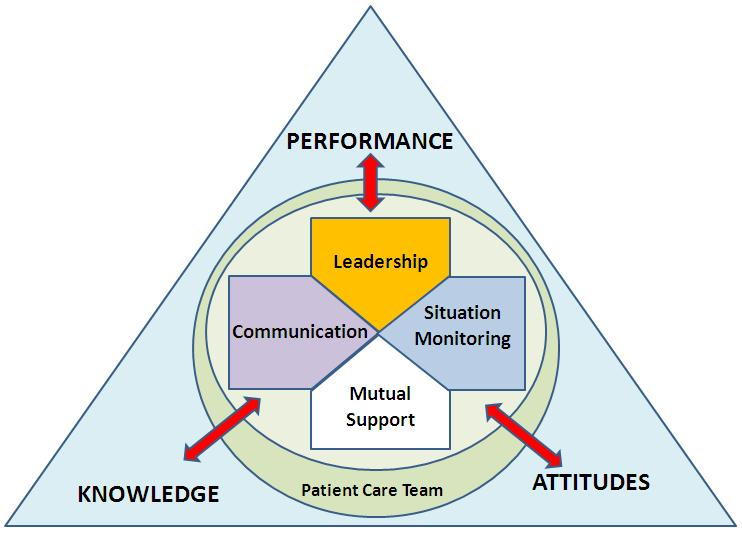
\includegraphics[width=0.35\textwidth]{TeamStepps.jpg}
  \end{center}
\vspace{-0.2in}
  \caption{\centering{\small{{\bf TeamSTEPPS:} Team Strategies and Tools to Enhance Performance and Patient Safety}}}
\vspace{-0.1in}
  \label{fig_cp}
\end{wrapfigure} 

The importance of studying a group of physicians entering a medical situation as a single operating unit began to appear in the focus of behavioral scientists with the publication of the Institute of Medicine (IoM) report titled \emph{To Err is Human: Building a Safer Health System} in Dec 1999. One of the four core messages from the report identified that patient life is lost not because of the failure of an individual, but due to the failure of the group as a whole. Since this report, Agency for Healthcare Research and Quality (AHRQ) and Department of Defense (DoD) have focused on the team failure from an Evidence-Based Medicine perspective and released Team Strategies and Tools to Enhance Performance and Patient Safety (TeamSTEPPS) [13] as the standard for team training in health care. The core of TeamSTEPPS focuses on the need to have (a) leadership, (b) mutual support, (c) communication, and (d) situation monitoring (or a shared mental model) among the team members, as shown in Figure 1.

The four team performance qualities identified above depends intricately on each medical personnel's communication abilities.  Behavioral psychologists have been studying the impact of socio-emotional states, especially stress induced socio-emotional states, on the performance of professionals and conclude that the direct artifact of stress include deprecated decision making, failure in leadership and breakdown of mutual support. Assessing the socio-emotional and communication skills of the professionals within the critical care unit will provide an unfettered advantage towards determining metrics of team performance under stress. To this end, in this paper we propose an initial set of three parameters that need to be studied towards advancing patient safety in critical care environments. Note that these research questions are still under investigation and their efficacy can only be hypothesized based on preliminary socio-behavioral studies conducted in related areas, under laboratory conditions.

\vspace{-0.1in}
\subsection{Automated monitoring of group dynamics to determine communication breakdowns}
\vspace{-0.13in}
Current team performance analysis systems are mostly based on retrospective video stream analysis collected during simulations of hospital emergency codes. The analyses are mostly based on expert’s opinion of what happened during critical incidents of the simulation [6] [3]. Unfortunately, expert’s time is very valuable and post-simulation analysis may not get sufficient attention due to increased hospital load. For long, researchers have questioned how communication between medical team members vary over the period of the emergency code execution [2], but very little is understood on the basics of the communication patterns during emergency, mostly due to the lack of automated annotation system that does not require expensive specialist time. Automated team performance analysis systems that focus on detecting specific instances of communication breakdown occurring during code simulation could greatly enhance our understanding of team work and how it can be enhanced through training. 

\vspace{-0.1in}
\subsection{Automatic evaluation of the social affinity between team members}
\vspace{-0.13in}
Sociograms (social affinity maps) have been used historically to determine the interpersonal match between members of a team or an organization. Sociograms are obtained through the process of sociometry [15], which quantitatively measures the relationships of individuals who exist within a social space. As mentioned earlier, in medical teams, the social space happens to be the emergency room where the team assembles with very little or no time to assess who are the members of the team. Sociometry is achieved through a set of evaluations that can assess the social interactions between individuals. The measurements could happen within the environment where the individuals interact (the medical team) or outside (casual interactions). Technologies developed to assess sociometric affinity between professionals could in turn provide quantitative evaluations of the social interactions between individuals. Sociograms developed at a hospital level could offer effective tools for quick team formations. Teams formed out of specialists, technicians and nurses who are closer to one another on the sociogram could offer a team with relatively less emotional stress. Socially closer individuals will also exhibit better communication, thereby increasing team performance. 

\vspace{-0.1in}
\subsection{Leadership evaluation and nomination through long term monitoring of individuals}
\vspace{-0.13in}
Theories of leadership have proposed evidence-based models for explaining qualities exemplified in successful leaders. Recently, the functional model of leadership [7] has been developed to describe team leaders as having self regulation which translates to learning, performance and adaptability. These models allow studying of dynamic teams that are formed in very short durations (like medical response teams) and allow monitoring of each individual and their contribution to the group activity.Reference [7] also describes a dynamic multi-goal model for team leadership which models effective leaders as those who can not only assess their own goals but also keep track of team goals, while approaching a dynamically evolving situation. Technologies developed towards understanding and modeling human interactions and communications can provide the tools needed to measure leadership qualities through long term monitoring.

\vspace{-0.1in}
\section{Conclusion}
\vspace{-0.2in}
In this paper, the importance of understanding and quantifying social interactions in both personal and professional environments are discussed in the context of multimedia, machine learning and pattern recognition perspectives. In the personal space, social interaction assistance was described within the constraints of developing a social interaction assistive technology, while in the professional space, some of the leading problems in medical team performance under stress was discussed in detail. While the first problem space discussed solutions that have already been proposed and field tested, the second problem still requires research towards understanding and appreciating the problem.



\subsubsection*{References}
\vspace{-0.11in}
\small{
[1] Balasubramanian V., Chakraborty S., Krishna S., Panchanathan S., "Human-Centered Machine Learning in a Social Interaction Assistant for Individuals with Visual Impairments", {\it Symposium on Assistive Machine Learning for People with Disabilities at Neural Information Processing Systems (NIPS)}, Dec 2009.\newline
[2] Bergs E., Rutten F., Tadros T., Krijnen P., and Schipper I., “Communication during trauma resuscitation: do we know what is happening?,” Injury,  vol. 36, 2005, 905-911.\newline
[3] Carbine D. N., Finer N.N., Knodel E., and Rich W., “Video recording as a means of evaluating neonatal resuscitation performance,” Pediatrics,  vol. 106, Oct. 2000,  654-658. \newline
[4] Gade L., Krishna S., and Panchanathan S. "Person localization using a wearable camera towards enhancing social interactions for individuals with visual impairment". {\it 1$^{st}$ ACM SIGMM international Workshop on Media Studies and Implementations that Help Improving Access To Disabled Users} MSIADU 2009, 53-62.\newline
[5] Humphrey N., “Vision in a monkey without striate cortex: a case study,” {\it Perception},  vol. 3, 1974, 241-255. \newline
[6] Karlgren N., Dahlström A., and Ponzer S., “Design of an Annotation Tool to Support Simulation Training of Medical Teams,” {\it Times of Convergence. Technologies Across Learning Contexts}, 2008, 179-184. \newline
[7] Kozlowski S.W.J., Gully S.M., McHugh P.P., Salas E., and Cannon-Bowers J.A., “A dynamic theory of leadership and team effectiveness: Developmental and task contingent leader roles.,” {\it Research in Personnel and Human Resources Management}, G. Ferris, Ed., JAI Press, 1996, 252-305. \newline
[8] Krishna S. and Panchanathan S., “Combining Skin-Color Detector and Evidence Aggregated Random Field Models towards Validating Face Detection Results,” in {\it  Indian Conference on Computer Vision, Graphics \& Image Processing}, 2008, 466-473. \newline
[9] Krishna S., Bala S., McDaniel T., McGuire S., and Panchanathan S., “VibroGlove: an assistive technology aid for conveying facial expressions,” { \it Proceedings of the 28th of the international conference extended abstracts on Human factors in computing systems}, Atlanta, Georgia, USA: ACM, 2010, 3637-3642.\newline
[10] Krishna S., Balasubramanian V., Panchanathan S., "Enriching Social Situational Awareness in Remote Interactions: Insights and Inspirations from Disability Focused Research, {\it ACM MM 2010 Brave New Ideas Session}, Oct 2010.\newline
[11] Krishna S., McDaniel T. and Panchanathan S., “Embodied Social Interaction Assistant”, {\it Technical Report \#TR-10-001}, Arizona State University, Tempe, 2010.\newline
[12] Krishna S., Panchanathan S., “Assistive Technologies as Effective Mediators in Interpersonal Social Interactions for Persons with Visual Disability,” {\it Computers Helping People with Special Needs}, Austria: Springer, 2010, 316 - 323. \newline
[13] Krishna S., Patel B., "Studying Individual’s and Group’s Scoio-Emotional Artifacts in Medical Teams towards Improved Patient Safety: A TeamSTEPPS Approach", {\it Technical Report \#TR-10-009}, Arizona State University, Tempe AZ USA July 2010. \newline
[14] McDaniel T., Krishna S. and Panchanathan S., “Using Tactile Rhythm to Convey Interpersonal Distances to Individuals who are Blind”, {\it Conference on Human Factors in Computing Systems}, 2009, 4669-4674. \newline
[15] Jennings H.H., {\it Sociometry in group relations}, 105th ed. (Washington): American Council on Education, 1959.

}

\end{document}
